\cleartorightpage
\setcounter{NAT@ctr}{-1}
\chapter*{}\label{chapter:vnmethod}

\begin{figure}[t!]
\centering

\includegraphics[height=10em]{frontmatter/images/chapter-header-variants.png}
\end{figure}
\vspace{-4cm}

\phantomsection\addcontentsline{toc}{section}{The Bio: Virtual Normal}
\articletitle{Discriminating somatic and germline mutations in tumor DNA samples without matching normals}\label{chapter:vnmethod-paper}

Saskia Hiltemann\textsuperscript{\ref{vn-affil:emc-bioinf}},
Guido Jenster\textsuperscript{\ref{vn-affil:emc-urology}},
Jan Trapman\textsuperscript{\ref{vn-affil:emc-pathology}},
Peter van der Spek\textsuperscript{\ref{vn-affil:emc-bioinf}},
Andrew Stubbs\textsuperscript{\ref{vn-affil:emc-bioinf}}

\small
\begin{enumerate}
\itemsep-0.5em
\item Department of Bioinformatics, Erasmus Medical Center, Rotterdam, The Netherlands. \label{vn-affil:emc-bioinf}
\item Department of Urology, Erasmus Medical Center, Rotterdam, The Netherlands \label{vn-affil:emc-urology}
\item Department of Pathology, Erasmus Medical Center, Rotterdam, The Netherlands. \label{vn-affil:emc-pathology}
\end{enumerate}

{\color{chaptergrey}{Published in:}} \emph{Genome Research}, 2015 Sep; 25(9): 1382–1390 \\
{\color{chaptergrey}{DOI:}} \hyperref[https://doi.org/10.1101/gr.183053.114]{10.1101/gr.183053.114}
% https://link.springer.com/article/10.1007/s10096-018-3220-z

\normalsize

\section*{Abstract}

Tumor analyses commonly employ a correction with a matched normal (MN), a sample from healthy tissue of the same individual, in order to distinguish germline mutations from somatic mutations. Since the majority of variants found in an individual are thought to be common within the population, we constructed a set of 931 samples from healthy, unrelated individuals, originating from two different sequencing platforms, to serve as a virtual normal (VN) in the absence of such an associated normal sample. Our approach removed (1) >96\% of the germline variants also removed by the MN sample and (2) a large number (2\%–8\%) of additional variants not corrected for by the associated normal. The combination of the VN with the MN improved the correction for polymorphisms significantly, with up to ∼30\% compared with MN and ∼15\% compared with VN only. We determined the number of unrelated genomes needed in order to correct at least as efficiently as the MN is about 200 for structural variations (SVs) and about 400 for single-nucleotide variants (SNVs) and indels. In addition, we propose that the removal of common variants with purely position-based methods is inaccurate and incurs additional false-positive somatic variants, and more sophisticated algorithms, which are capable of leveraging information about the area surrounding variants, are needed for optimal accuracy. Our VN correction method can be used to analyze any list of variants, regardless of sequencing platform of origin. This VN methodology is available for use on our public Galaxy server.

\section*{Introduction}

Analysis of 1092 human genomes performed by the 1000 Genomes Project reveals that an individual has approximately 4 million variations (on average, 3.7 million SNPs, 350,000 insertions and deletions [indels], and 750 large deletions) compared with the reference genome and that the vast majority of an individual's germline variations are polymorphic within the human population, with >95\% of all single-nucleotide variants (SNVs) and small indels in a given individual occurring at a frequency of ≥0.5\%~\cite{10002010map,10002012integrated}. Therefore, whenever a matched normal (MN) sample was unavailable (most commonly due to lack of funds or sample availability), researchers have typically relied on the public mutation databases and/or a set of in-house genomes for the filtering of germline variants from the full set of variants found in a tumor sample~\cite{yoon2009sensitive,kumar2011exome}. In recent years, these catalogs of human variation have grown exponentially, causing some researchers to question the necessity of sequencing a MN control for every tumor sample~\cite{kumar2011exome}.

In this study, we address the questions of whether current mutation databases are complete enough to correct for common and rare polymorphisms and of how well this filtering performs compared with the correction with a MN sample.

There are many public databases of human variation available. The Single Nucleotide Polymorphism Database (dbSNP) is a free public archive for genetic variation within and across different species~\cite{sherry2001dbsnp}. Its latest build (138) contains over 63 million polymorphisms found within the human population. The 1000 Genomes Project (1000G) database contains polymorphisms encountered in a set of 1092 genomes of healthy individuals~\cite{10002010map,10002012integrated}. The NHLBI Exome Variant Server (EVS) contains exonic variants from over 6500 genomes (\url{http://evs.gs.washington.edu/EVS}).

In an effort to improve the control-free correction method further, we constructed what we call a virtual normal (VN). This is a set of 931 samples from healthy, unrelated individuals, whole-genome sequenced to high depth, originating from two different sequencing platforms. Our VN consists of 433 public samples from Complete Genomics~\cite{drmanac2010human}, sequenced in the context of the 1000G, as well as 498 samples sequenced on Illumina HiSeq technology by the Genome of the Netherlands (GoNL) Consortium~\cite{boomsma2014genome,francioli2014whole}.

For copy-number analysis of sequencing data, tools exist that correct for normal contamination in unmatched tumor samples~\cite{boeva2010control}. The idea of using a set of genomes for correction of copy-number variants has also been described~\cite{yoon2009sensitive}. Apart from a correction based on GC content, this read-depth method also corrects for regions found to have an increased or decreased copy number across all five of their samples (from healthy individuals) and therefore likely a polymorphism within the population. We aim to assess the validity of such an approach and extend it by applying it to structural variation (SV), as well as SNV and indel analysis, in whole-genome-sequenced cancer samples. Additionally, we investigate the minimal size of such a VN necessary for adequate filtering and assess the influence of different ethnicities within the set.

Variants in mutation databases are usually represented only by their position relative to the reference genome and the variant allele, as well as possibly a quality metric. The advantage of using a VN is that we can also leverage information about the area surrounding a variant (e.g., nearby variants in the same sample) to optimize correction. There are often several different ways to describe the same variant, possibly involving (slightly) different chromosomal positions, which means that comparison methods that require an exact match of position and variant nucleotides may be suboptimal, leading to false-positive somatic variants. The algorithm we use with our VN correction is capable of detecting equivalences of differently described variants by taking into account the reference sequence surrounding a variant, as well as neighboring variants. This provides a valuable improvement over correction using variant databases, where this contextual information is lost.

\section*{Results}

We evaluate the performance of the different correction methods on four tumor-normal pairs from two different tumor types (breast and prostate cancer). All of the samples were sequenced by Complete Genomics. Two of the samples were also sequenced using Illumina technology. We evaluate the correction of SNVs and indels of up to ∼50 bp, as well as the larger SVs. For the breast cancer samples, additional validation data were available from the COSMIC database, and we used these confirmed variants to assess the performance of the three different correction methods (MN, mutation databases, VN).

We have made our VN correction method available as a tool for the Galaxy workflow platform~\cite{giardine2005galaxy,blankenberg2010galaxy2,goecks2010galaxy} as part of our tumor analysis in Galaxy (TAG) tool suite~\cite{hiltemann2014cgtag}.

\subsection*{MN vs. VN}

We use three correction methods in order to determine the set of tumor-specific (somatic) variants: a correction for germline variants using a MN sample, a correction for polymorphisms using the VN, and a correction for polymorphisms using public mutation databases (dbSNP, 1000G, and EVS). All variants remaining after application of all three correction methods represent the (consensus) set of true somatic variants. A false-positive variant of a method is any variant remaining after correction, which would have been removed had we employed all three correction methods.

\subsection*{Structural variations}

There are far fewer common SVs, than SNVs and indels, present in public databases. And the few sources of common SVs contain almost exclusively copy-number variants (large indels) and almost none of the more complex SVs such as inversions and translocations. This makes filtering of tumor variants when there is no MN sample very challenging. The Database of Genomic Variants (DGV)~\cite{macdonald2013database} is currently the largest SV database, with approximately 200,000 variants. However, >99\% of these variants are copy-number changes (gains or losses), and the database contains only a limited number of the more complex structural variant types such as inversions and (balanced) translocations, while these are thought to be common in the normal population~\cite{feuk2006structural,10002010map,10002012integrated,mills2011mapping}. We additionally filtered using BreakSeq database~\cite{lam2010nucleotide}, BreakDB~\cite{korbel2009pemer}, and the 1000G SVs~\cite{10002010map,10002012integrated}, which collectively contain another 32,000 structural variants.

We compared the SVs found in the tumor sample to those in the online databases and the VN\@. We consider two SVs a match if both sides of the event occur within a small distance of the sides of the other SV (200 bp when originating from the same platform, 500 bp when cross-platform).

In the Complete Genomics samples, the VN method removed most of the germline structural variants also removed by the associated normal (∼97\%) while also removing a further 6\%–8\% of common variants not corrected for by the associated normal.

For the Illumina samples, the VN method removed fewer SVs than the MN but was still a huge improvement over using only the database filter. The Illumina HCC1187 sample had 132,045 SVs identified in the tumor sample, of which 1464 were of high quality (QUAL ≥ 200). By use of the VN filter, we removed 961 polymorphic variants from this list (\hyperref[fig:svcomparison]{Fig.~\ref{fig:svcomparison}}). Increasing the distance parameter further (to 2000–5000 bp) resulted in the filtering of more SVs than the MN.

\begin{figure}[t!]
\centering
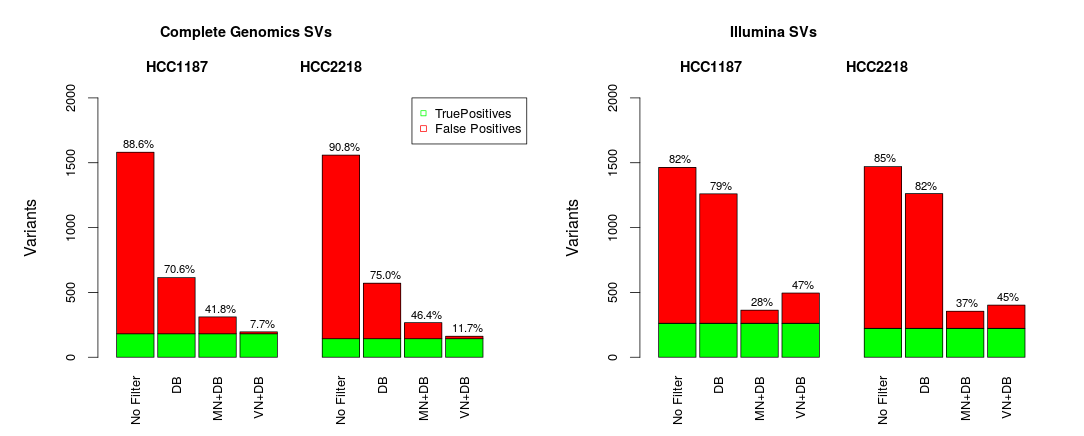
\includegraphics[width=\textwidth]{chapters/images/virtualnormal/Hiltemann_Figure1.png}
\caption{\textbf{Comparison of matched normal (MN) and virtual normal (VN) methods for structural variations (SVs).} Correction of high-confidence SVs from Complete Genomics (left) and Illumina (right), using the database filter (DB), MN, and VN\@. Light gray area indicates the golden set (combination of the three).}
\label{fig:svcomparison}
\end{figure}

Experimental validation data for the two public genomes HCC1187 and HCC2218 were obtained from the COSMIC database~\cite{forbes2010cosmic,bindal2011cosmic}. We determined the number of these confirmed somatic SVs detected in each sample and determined the number of detected SVs that survived our correction method (\hyperref[table:table1]{Table~\ref{table:table1}}). The CG samples had higher sensitivity (detected more of the validated SVs), but for every tumor sample, those variants that were detected by the platform and determined somatic after correction with the MN all survived correction with VN and DB.

\small
\begin{table}[t!]
\centering
\begin{tabular}{lllll}
          & Sample  & Detected & Somatic & Description of variants called somatic \\ \hline
Illumina  & HCC1187 & 71 of 98 & 53 & 53 of 71 matches survived MN correction; \\
          &         &          &    & all of these survived DB+ VN correction \\
Illumina  & HCC2218 & 54 of 64 & 10 & 10 of 54 matches survived MN correction;\\
          &         &          &    & all of these survived DB+ VN correction \\
CG        & HCC1187 & 91 of 98 & 91 & All survived MN correction; \\
          &         &          &    & all of these survived DB+ VN correction \\
CG        & HCC2218 & 55 of 64 & 55 & All survived MN correction; \\
          &         &          &    & all of these survived DB+ VN correction \\
\end{tabular}
\caption{Number of confirmed somatic SVs (as described in COSMIC database) detected in the tumor samples by CG and Illumina, and the number of these variants that are labeled soatic after corrections with our VN method}
\label{table:table1}
\end{table}
\normalsize

\subsection*{SNVs and indels}

For the analysis of SNVs and indels for both the MN method and the VN method, we additionally filter variants for their presence in dbSNP~\cite{sherry2001dbsnp}, the 1000G~\cite{10002010map,10002012integrated}, and the EVS (\url{http://evs.gs.washington.edu/EVS}) using the ANNOVAR tool~\cite{wang2010annovar}.

In annotating with the online databases, we require an exact match of position, as well as a match in variant allele between the cancer sample and the variant described in the database. For dbSNP, we used the set of nonflagged variants (flagged variants are those for which SNPs <1\% minor allele frequency [MAF; or unknown], mapping only once to reference assembly, or flagged as “clinically associated”).

The Illumina FastTrack Cancer Service (\url{http://www.illumina.com/services/whole-genome-sequencing-services/sequencing-service-providers-ign/sequencing-services.ilmn}) identified 15,499 somatic SNVs in the HCC1187 sample and 27,823 in HCC2218, after correction with the MN sample. We evaluate performance of our method by correcting the list of all variants found in the tumor sample using our VN set and comparing the remaining variants to those variants determined to be somatic by Illumina's tumor-normal sequencing service.

Two variants are considered a match when they share the same chromosomal position, as well as the same variant allele. Because variants can often be described in various different yet equivalent ways, we used a more advanced correction method for those comparisons involving CG data (the TestVariants tool from CG's tool suite). Detecting these equivalencies is very important for variant comparisons and is discussed in more detail in a later section.

Variants remaining after application of all three filters (MN, database filter, and VN) represent the golden set of true somatic variants (11,409 SNVs for HCC1187 and 20,560 for HCC2218). We determined the number of false-positive somatic variants identified by several filter combinations (\hyperref[fig:snvcomparison]{Fig.~\ref{fig:snvcomparison}}; \href{https://genome.cshlp.org/content/25/9/1382/suppl/DC1}{Supplemental Data S2}). High-confidence variants determined by the VN method are those variants not present in any of the VN samples, and the position may not be no-called in more than ∼50\% of the samples. This is similar to the MN correction, where typically only those variants are reported that were called reference in the normal sample; tumor variants at positions that are no-called in the normal are usually not reported as (high-confidence) somatic variants.

The VN approach has similar performance to a MN for SNVs and indels and even removes more variants than the associated normal in some cases (\hyperref[fig:snvcomparison]{Fig.~\ref{fig:snvcomparison}}). However, be aware that this does not mean it removes all of the same variants as the normal but rather it removes an equally large, but different set of variants. There are always highly personal germline variants that can only be removed by the MN, but similarly, there are also polymorphisms that are only removed by the VN and not the single MN sample.

\begin{figure}[t!]
\centering
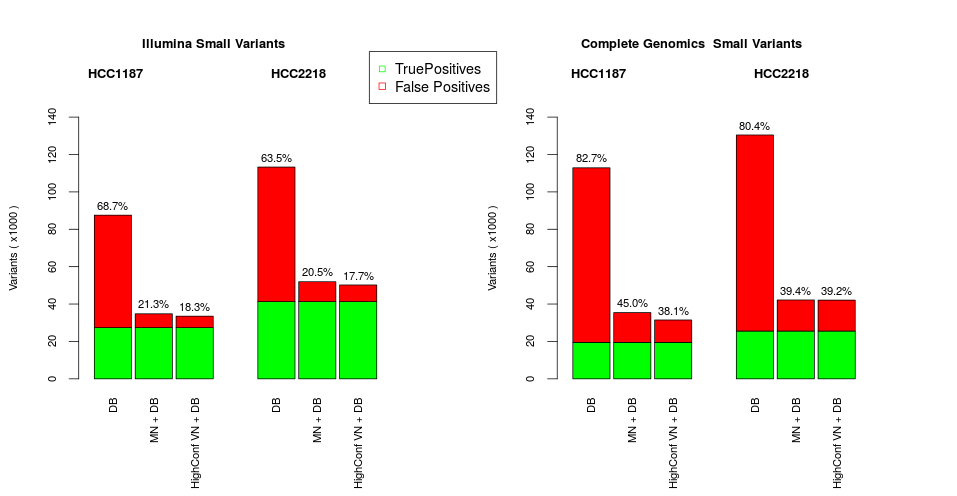
\includegraphics[width=\textwidth]{chapters/images/virtualnormal/Hiltemann_Figure2.png}
\caption{\textbf{Number of false-positive SNVs and indels identified per filtering method for Illumina (left) and Complete Genomics (right).} True positives (green) are those variants remaining after application of all filters (for VN, we did not use the high-confidence criterion to determine the set of true positives). DB denotes an aggressive database filter. HighConf VN+DB denotes the list of high-confidence somatic variants as determined by the VN and database filters. MN + DB denotes the list of high-confidence somatic variants after correction with a MN combined with the database filter. }
\label{fig:snvcomparison}
\end{figure}

Significant improvement is made over the situation where no MN is available and only aggressive filtering with public databases is used. The advantage of using a VN method rather than relying solely on databases is greatest for indels, which are less abundant in the public databases than SNVs and are more difficult to annotate using a purely position-based method because they can often be called in various different but equivalent ways.

To ascertain the quality of the somatic variants identified by our method, we determined several metrics such as Ti/Tv ratio (\href{https://genome.cshlp.org/content/25/9/1382/suppl/DC1}{Supplemental Data S3}). We see that the Ti/Tv ratio decreases as more filtering is performed, which is expected for the tumor-specific mutations, as these are more random in nature. Breast cancer specifically has been shown to favor transversion variants~\cite{liu2002genetic}. Mutational spectra of the somatic variants determined by our method were also investigated (\href{https://genome.cshlp.org/content/25/9/1382/suppl/DC1}{Supplemental Data S3}) and are consistent with the literature~\cite{rubin2009mutation} in terms of mutation patterns.

Validation data were obtained from COSMIC for both samples. We used this list to determine the number of these validated variants that were detected in the tumor samples by each platform and to determine how many survived correction by our VN method (\hyperref[table:table2]{Table~\ref{table:table2}}). Over 94\% of the validated variants were detected in each tumor data set, and of the detected variants, only one variant in one of the samples was filtered out only by the VN, indicating a possible false-negative of our method. One confirmed somatic variant in the HCC1187 sample (both Illumina and CG) was present in the associated normals, the public databases, and the VN (17 samples), indicating a possible false positive in the COSMIC database. One of the confirmed variants in COSMIC for the HCC2218 sample appeared in our VN nine times, as well as in the dbSNP, the EVS, and 1000G, for both Illumina and CG, indicating another possible false positive in COSMIC\@. For each of the samples, five confirmed somatic variants were present in the dbSNP (NonFlagged) database. These variants were not present in the VN, the 1000G data, or the EVS and thus are likely disease-related variants that should have been flagged in dbSNP but were not.

\small
\begin{table}[t!]
\centering
\begin{tabular}{lllll}
          & Sample  & Detected   & Somatic & Description of variants called somatic \\ \hline
Illumina  & HCC1187 & 82 of 86   & 75      & Five filtered by dbSNP; one by VN only(1x); \\
          &         &            &         & 1 N + DB + VN(17x) \\
Illumina  & HCC2218 & 178 of 182 & 172     & Five filtred by dbSNP; one in DB (dbSNP + \\
          &         &            &         & 1kG + EVS) +VN(19x)\\
CG        & HCC1187 & 82 of 86   & 76      & Five filtered by dbSNP;\\
          &         &            &         & one N + DB + VN(17x); \\
CG        & HCC2218 & 173 of 182 & 167     & Five filtered by dbSNP; one in DB (dbSNP + \\
          &         &            &         & 1kG + EVS) + VN(9x) \\
\end{tabular}
\caption{Number of confirmed somatic variants (as described in COSMIC database) detected in the tumor samples by CG and Illumina, and the number of these variants that are labeled soatic after corrections with our VN method}
\label{table:table2}
\end{table}
\normalsize

\subsection*{Size of VN}

\subsubsection*{Structural variations}
We determined the number of VN samples required for filtering of common germline SVs for each sample (\hyperref[fig:vnsize]{Fig.~\ref{fig:vnsize}}). For the Complete Genomics samples, after using about 50 VN samples, the same numbers of SVs are filtered out as when using the MN\@. A plateau is reached after about 120 VN samples, and adding additional normal samples filters out only a small number of additional SVs. Correction with the VN did not remove as many variants as the MN for the Illumina sample, though it still provides significant improvement over filtering with databases alone. A plateau is also reached for the Illumina samples at around 300 VN samples. Increasing the distance threshold for when to consider two SVs a match to 2000 - 5000 bp did result in correction of the same number of SVs as the MN but is likely less accurate.

\begin{figure}[t!]
\centering
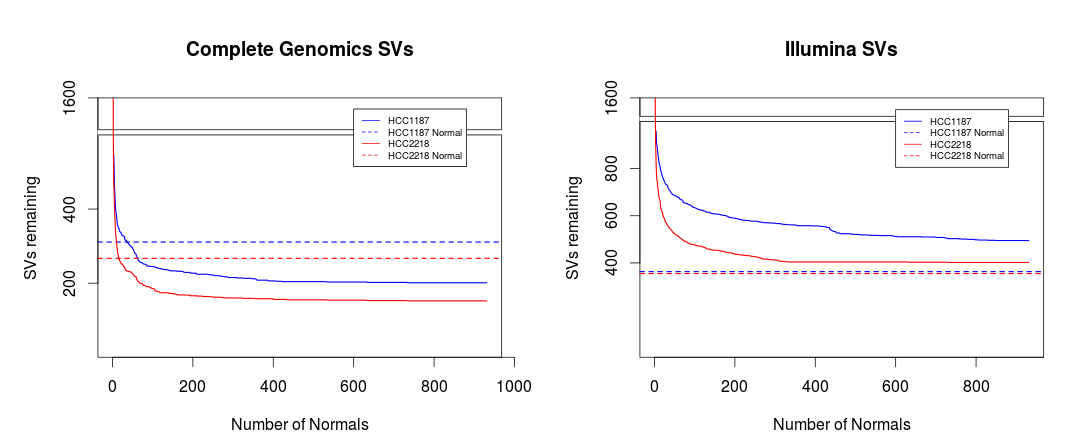
\includegraphics[width=\textwidth]{chapters/images/virtualnormal/Hiltemann_Figure3.png}
\caption{Number of structural variants filtered out after each additional VN sample for Complete Genomics (left) and Illumina samples (right). Blue denotes the HCC1187 sample; red, CG HCC2218. Dashed lines indicate the level reached by correction with the associated normal. }
\label{fig:vnsize}
\end{figure}

\subsubsection*{SNVs and indels}
We investigated how many VN samples are necessary for adequate filtering (\hyperref[fig:vnsize2]{Fig.~\ref{fig:vnsize2}}). We are able to attach a confidence measure to the remaining somatic variants by determining the number of VN samples that are no-called at the variants’ locus (e.g., a variant at a position that was fully called reference in all 931 normals is more likely to be a true somatic variant than a variant that was also not detected in any of the VN samples but no-called in all normals).


\begin{figure}[t!]
\centering
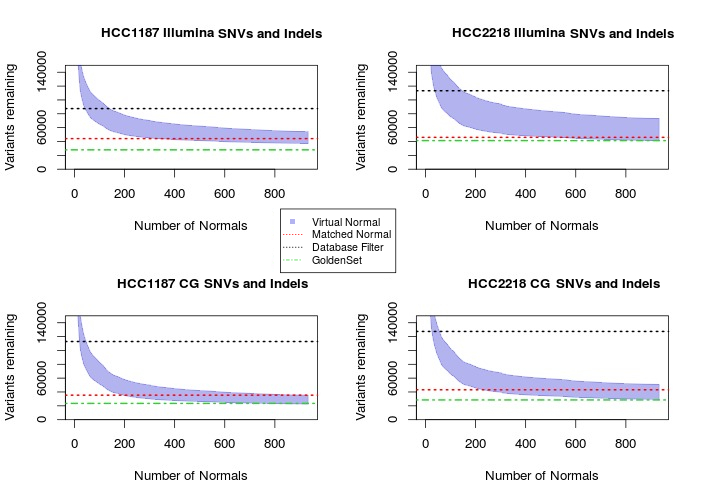
\includegraphics[width=\textwidth]{chapters/images/virtualnormal/Hiltemann_Figure4_fixed.jpg}
\caption{\textbf{Number of SNVs and indels removed after filtering with each additional VN sample.} Black dashed line indicates the number of variants labeled as somatic when using only a database filter; red dashed line, the number of variants after correction with MN and the public databases; and the green dashed line, the golden set variants, those remaining after application of all correction methods. The shaded area indicates the number of variants remaining after VN filtering, ranging from all variants (upper bound) to highest-confidence somatic variants (lower bound).}
\label{fig:vnsize2}
\end{figure}

The SNV and indel analysis results separated by variant type are presented in \href{https://genome.cshlp.org/content/25/9/1382/suppl/DC1}{Supplemental Data S8}. The advantage of the VN method over a database correction was greatest for indels, likely due the fact that these variants can more often be described in various different ways and at slightly different positions and therefore benefit more from the enhanced correction algorithm used in our method than the SNVs. For both SNVs and indels, the number of variants removed is comparable to the number removed by the MN and is significantly more than database corrections alone.

Analysis of SNVs revealed that for the CG samples, about 200 samples are needed to obtain the same performance as using the online databases alone, and any additional genomes added beyond that point will improve the filtering of common variants even further. The Illumina samples required a greater number of CG normals, about 300. For indel variants, the number of normal needed to surpass performance of the online databases alone is fewer than 100 for both platforms. Indel variants can more often be described in different but equivalent forms than SNVs, which means they benefit most from the enhanced comparison method used in our VN approach. The performance is better for Complete Genomics samples than for Illumina samples, but for both platforms, the performance is significantly improved by not relying solely on public mutation databases.

\subsection*{Prostate Cancer Samples}
ince HCC1187 and HCC2218 samples are both cell lines, we analyzed two prostate cancer patient samples, G110 and G316, to demonstrate that our method also works for patient data. The results are described in more detail in the \href{https://genome.cshlp.org/content/25/9/1382/suppl/DC1}{Supplemental Data S7}. These two samples were sequenced by Complete Genomics and use genome build hg18. Out of our 931 VN samples, 85 were also available on hg18, so for this analysis we used a smaller VN\@. Despite this reduced number of normals, our method could still correct as many variants as the MN, requiring around 60–100 normals genomes to do so (20–40 for SVs).


\subsection*{Influence of ethnicity}

The influence of ethnicity on the correction power was checked for 54 VN genomes from the Complete Genomics’ diversity panel. This panel contains individuals from five different populations across the world. We found that while there was a clear difference between genomes from different races, this difference was <10\%, and the set as a whole is capable of correcting as efficiently as a MN regardless of the background of the individual (\href{https://genome.cshlp.org/content/25/9/1382/suppl/DC1}{Supplemental Data S6}).

\subsection*{Improved correction method}

When comparing the variants found in a (tumor) sample to lists of known polymorphisms, the method most often used is to compare start and end coordinates of the two variants, as well as the observed sequence, and if these three values are identical, the variants are considered equal. However, this approach may be too naïve as there are often various different ways of describing the same variant, depending on the surrounding (reference) sequence and nearby variants.

Consider the following very simple example: Given a reference sequence of CAG and a variant sequence of CAAG, do we describe the variant as an A having been inserted after the C or before the G? Both descriptions are equally valid, but the position of the inserted nucleotide will differ by one. There is no real community consensus on how to resolve these kinds of canonicalization issues, though left alignment is by far the most commonly used. However, the HGVS recommendations urge \textit{“for all descriptions [to use] the most 3′ position possible”}, which would imply right alignment of variants on forward strand genes (\url{http://www.hgvs.org/mutnomen/recs-DNA.html}).

Another example, and one of the most frequently observed types of annotation difficulties in our data sets, are so-called block substitutions. Whenever two SNVs occur within a 3-bp window and are observed on the same reads, Complete Genomics will call a single 2- or 3-bp substitution, while Illumina will simply call two SNVs. Complete Genomics chooses this approach in order to retain the knowledge that these two variants were encountered on the same allele and possibly within the same codon, which is important for the determination of the impact of the variant on the protein. While the observed sequence for both platforms was the same, the descriptions differ, and naïve comparison methods will not be able to detect the equivalence of these variants.

We identified four main classes of equivalent, but differently described SNVs and indels in our data sets:

\begin{enumerate}
\item \textbf {Multivariants.} A series of nearby SNVs and indels may also be described as a single, larger substitution in order to retain the knowledge that they occurred on the same allele. The block substitutions are an example of this class (\hyperref[fig:variantannotation]{Fig.~\ref{fig:variantannotation}A}).

\item \textbf{Subvariants.} A variant is present in both samples, but in one of the samples, it was adjacent to another variant so in that sample the variant was part of a larger variant (\hyperref[fig:variantannotation]{Fig.~\ref{fig:variantannotation}B}).

\item \textbf{Canonicalization.} The same variant sequence is observed in both samples, but it can be described at a different position and possibly with a different observed variant sequence (\hyperref[fig:variantannotation]{Fig.~\ref{fig:variantannotation}C}).

\item \textbf{Annotation issues.} Different variant callers and different file formats will have differences in the way they describe variants; for example, when there are multiple variants at the same locus, the descriptions in the VCF format will be different than had the variants occurred alone, turning SNVs into multinucleotide variants and turning simple indels into complicated descriptors (\hyperref[fig:variantannotation]{Fig.~\ref{fig:variantannotation}D}). For example, in the Illumina VCF files, variants of the following pattern are frequently observed: TCA → TA,TC\@. This indicates that on one allele, the C nucleotide was deleted; on another, the A nucleotide. However, had only the deletion of A occurred, the variant would have been described as CA → C, and thus, the position of the variant would also have been shifted by one. Similarly, had only the deletion of C occurred, the description of the variant would have been TC → T, with an unchanged position field. Many tools converting VCF to a one-line-per-variant format simply split on the comma (TCA → TA and TCA → TC). While it is usually not difficult to reduce these variants to their canonical forms, many tools do not handle this issue correctly, and databases may not always ensure that only canonical forms are entered.
\end{enumerate}

\begin{figure}[t!]
\centering
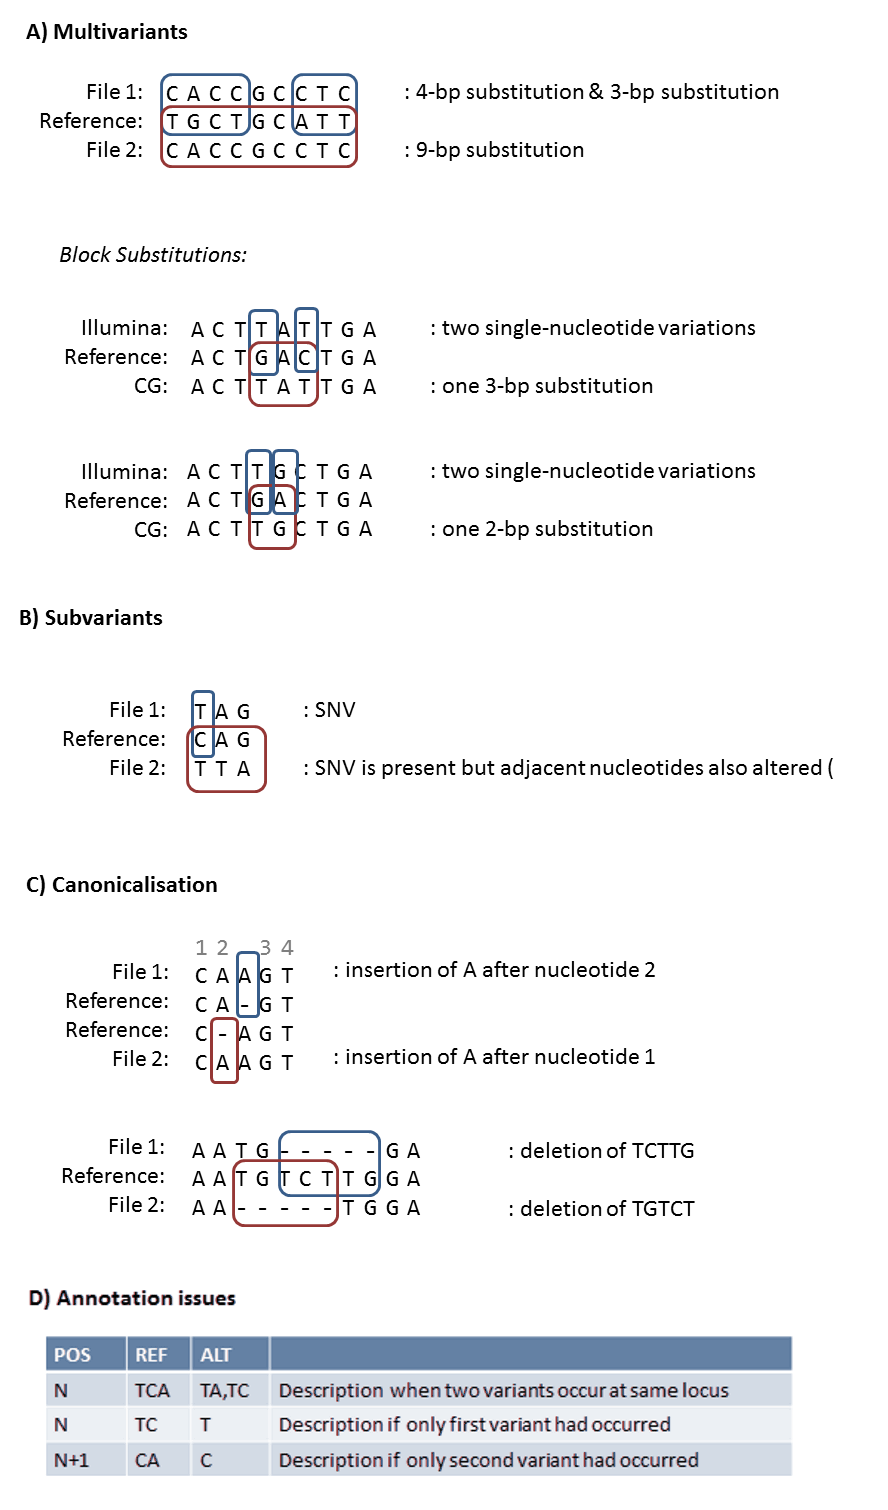
\includegraphics[width=0.6\textwidth]{chapters/images/virtualnormal/Hiltemann_Figure5.png}
\caption{\textbf{Examples of equivalent, but differently annotated variants.} (A) When several nearby bases are changed, this can be described as one large substitution or as several smaller ones, even though the resulting sequence is the same. (B) Variant was present, but changes were described as part of a larger variant. (C) Canonicalization issues: Variants can often be described at various different positions, and variants originating from different sources may use different conventions, which must be taken into account during comparisons. (D) In the VCF format, overlapping variants can result in a different description of variants than had they occurred in isolation, a subtlety not always dealt with correctly in comparison algorithms. }
\label{fig:variantannotation}
\end{figure}

When comparing variants originating from the exact same sequencing and processing pipelines, these issues are minimal, but when comparing variants from different sources, they become more pronounced and must be dealt with in order to maximize the utility of variant databases. We encountered these problems many times when doing comparisons to COSMIC variants and describe several examples in more detail in \href{https://genome.cshlp.org/content/25/9/1382/suppl/DC1}{Supplemental Data S4}.

The comparison algorithm we use for our VN correction (CGATools) is capable of detecting most of these equivalences between SNVs and indels and therefore reduces the number of false-positive somatic variants identified.

The description of SVs is even less standardized, making comparisons of variants originating from different sources even more challenging. The differences in calling conventions for SVs are discussed in \href{https://genome.cshlp.org/content/25/9/1382/suppl/DC1}{Supplemental Data S4}.

\subsection*{Tumor analysis in Galaxy}

Galaxy is a free and open-source web-based analysis platform for data intensive biomedical research~\cite{giardine2005galaxy,blankenberg2010galaxy2,goecks2010galaxy}. Our VN filtering method is available as a tool for the Galaxy platform as part of our TAG tool suite. The tool can be installed to a local Galaxy instance via the DTL (Dutch Techcenter for Life Sciences) tool shed (\url{http://toolshed.dtls.nl}). Additional normal samples can easily be added to the VN set in this tool. Further installation and usage instructions can be found within the tool's tool shed repository. The tools have been installed on our demo galaxy example (\url{http://galaxy-demo.ctmm-trait.nl/u/saskia-hiltemann/p/virtual-normal-analysis})~\cite{hiltemann2014cgtag}; however, due to limited resources, we have had to impose disk and job quotas and recommend installing the tool onto a local (production) Galaxy server for optimal performance. Information about installing and maintaining a Galaxy server is available from the Galaxy wiki (\url{http://galaxyproject.org}).

\section*{Discussion}

We have developed a method for the filtering of tumor variants in the absence of a MN sample. To this end, we have constructed a VN consisting of a set of 931 whole genomes from healthy, unrelated individuals (433 sequenced by Complete Genomics, 498 by Illumina). We evaluated our method on four tumor-normal pairs of two different cancer types, from two different sequencing platforms (CG and Illumina), for both SVs and SNVs and indels. We found that such a VN can correct as many variants as a MN (and in many cases even more), allowing it to possibly serve as a substitute for a MN sample in a research context or provide a valuable addition to the MN in a more clinical setting where highest accuracy is required. It offers a huge improvement over the use of public databases alone, for example, in situations where no normal tissue is available.

Germline variations detected in these tumors after correction with associated normal are in the range of 80\%–85\% for SVs and 90\%–96\% for SNVs and small indels and substitutions. Our VN method is able to filter out most of these germline variants (96\%–99\%) and removes a large number of additional common variants not detected by the associated normal sample. The consensus set of variants—those remaining after correction with associated normal, VN, and public mutation databases—represents the set of true somatic variants. Our method identifies ∼10\%–30\% false-positive SVs and 20\%–30\% false-positive SNVs and indels, while the tumor-normal method has ∼20\%–50\% and 40\%–45\% false positives for SVs and SNVs and indels, respectively. This suggests that a VN could act as a substitute for an associated normal when the latter is unavailable, and even outperforms the standard MN correction in terms of false-positive rate in some samples.

The reason for the observation that correction using a VN collection can outperform the MN could be that the sequencing of a single MN sample will not call all germline variants. At the moment with an approximately 100× coverage single-sample analysis by Complete Genomics, ∼2.5\% of bases (∼70,000,000 bases) are not called. If these noncalls are random, a collection of samples will always outperform the correction using a single control. Therefore, we conclude that at the current coverage of 100× or less, a single normal matched control for correction of germline variants should be supplemented with (or even replaced by) a series of at least 200 control genomes in order to deliver optimal results.

We also investigated the optimal size of the VN set and determined that approximately 200–400 genomes are required in order to correct at least as efficiently as the MN sample for SNVs (fewer were required for CG-sequenced samples, as our VN also consisted of CG-sequenced samples). For SVs, 10–40 genomes were required for the CG samples, and for the Illumina samples, our 433 VN samples corrected fewer variants than the associated normal, largely owing to the fact that the description of breakpoints differs so greatly between the two platforms; were we to construct a VN of Illumina-sequenced samples, results would likely vastly improve.

Furthermore, we argue that using a purely position-based annotation incurs additional false positives, should be replaced by an algorithm capable of detecting the equivalence of variants called in different forms, and has knowledge of the reference genome and other nearby variants. When comparing variants obtained from the same sequencing platform and called using the same algorithm, a purely position-based method could suffice, but public databases often contain variants from various sources and are called using various different (versions of) algorithms; in order to utilize the full power of these databases, algorithms need to be able to detect equivalence of variants called in different forms and/or at different locations.

Some caveats to this approach exist: a VN approach cannot correct for those germline variants that are highly personal. Therefore, additional care must be taken when submitting variants to public databases to ensure the anonymity of the patient. In addition, the possibility exists that by foregoing the sequencing of a normal sample, rare germline variants may be mistakenly labeled as somatic, which may lead to rare heritable mutations being overlooked. Additional validation of the somatic status of the variants may be desirable in these cases, either by work in the laboratory or by considering larger groups of patients.

We are able to attach a confidence measure to the somatic variants as determined by our VN method by considering the number of VN samples that are no-called at the variants’ loci. A somatic variant at a position that was fully called reference in all 931 normals is more likely to be a true somatic variant than a variant that was also not detected in any of the VN samples but was no-called in all normal samples (i.e., evidence of absence vs.\ absence of evidence). Currently, this could only be done for the VN samples sequenced by CG, as the Illumina data does not provide the necessary information about no-called and half-called loci.

Our VN correction with the 931 samples can be run on any VCF file or list of variants, regardless of the sequencing platform of origin, and is available as a Galaxy tool from the DTLS tool shed (\url{http://toolshed.dtls.nl/repos/saskia-hiltemann/virtual\_normal\_preprocessing}) and is installed on our public demonstration Galaxy server (\url{http://galaxy-demo.ctmm-trait.nl}).

\section*{Methods}

\subsection*{Illumina vs. Complete Genomics}

For this study we analyzed two breast cancer cell line samples, HCC1187 and HCC2218, which have been whole-genome-sequenced by both Complete Genomics and Illumina and are publicly available for download (\url{ftp://ftp2.completegenomics.com/Cancer\_pairs/} and \url{https://basespace.illumina.com/datacentral}).

Comparisons between the Illumina and Complete Genomics platforms have been previously described~\cite{lam2012performance}. We compared the variants identified by each of the platforms for our samples and found that >96\% of the SNVs and >70\% of the indels identified by Complete Genomics were also present in the Illumina samples (\href{https://genome.cshlp.org/content/25/9/1382/suppl/DC1}{Supplemental Data S1}).

The description of SVs differs greatly between the two platforms, making comparison a challenging task. Our algorithm found an overlap of ∼40\%–45\% (\href{https://genome.cshlp.org/content/25/9/1382/suppl/DC1}{Supplemental Table S1.3}). The calling differences and comparison pitfalls are discussed in a later section.

\subsection*{Complete Genomics samples}

The HCC1187 breast cancer (primary ductal carcinoma) sample was TNM stage IIA, grade 3. For HCC1187 BL, the normal sample was derived from peripheral blood and immortalized with EBV transformation. ATCC numbers were as follows: tumor, CRL-2322; normal, CRL-2323. CG Software version used was 2.0.2.15.

The HCC2218 breast cancer (primary ductal carcinoma) sample was TNM stage IIIA, grade 3. For NA12880, the normal sample was derived from peripheral blood and immortalized with EBV transformation. ATCC numbers were as follows: tumor, CRL-2343; normal, CRL-2363. CG Software version used was 2.0.2.15.

Samples have been sequenced to an average genome-wide coverage of 123× for three of the samples and 92× for the NA12880 sample. The HCC1187 and HCC2218 samples were downloaded from Complete Genomics (\url{ftp://ftp2.completegenomics.com/Cancer\_pairs/}).

The prostate cancer sample G110 is derived from a radical prostatectomy. The tumor section from which DNA was isolated had a Gleason score of 3 + 3 and contained 80\% epithelial tissue, of which 90\% was cancer. The MN DNA was isolated from peripheral blood. The G110 and MN samples were sequenced by Complete Genomics to an average genome-wide coverage of 94× and 109×, respectively. The software version used was 2.0.2.24.

The prostate cancer sample G316 is derived from a transurethral resection of the prostate (TURP). The tumor section from which DNA was isolated had a Gleason score of 4 + 3 and contained only epithelial tissue, of which 100\% was cancer. The MN DNA was isolated from peripheral blood. The G316 and MN samples were sequenced by Complete Genomics to an average genome-wide coverage of 112× and 113×, respectively. The software version used was 2.0.2.24.
VN samples

The 433 normal samples were sequenced by Complete Genomics in the context of the 1000G and are accessible for download from the EBI and NCBI ftp servers at \url{ftp://ftp.1000genomes.ebi.ac.uk/vol1/ftp/} or \url{ftp://ftp-trace.ncbi.nih.gov/1000genomes/ftp/}.

For the hg18 prostate cancer samples, our VN set contained 66 normals, consisting of (1) the Complete Genomics diversity panel (46 genomes), (2) the four unrelated individuals from the CG pedigree, (3) the parents in the two CG trios (YRI and PUR), and (4) 12 in-house samples of healthy, unrelated individuals. This amounts to a total of 66 genomes. For the SNV and indel analysis, an additional 19 in-house samples were available, bringing the total up to 85. The Complete Genomics public samples may be downloaded from \url{ftp://ftp2.completegenomics.com/}. A list of all variants found in our in-house VN samples is available as a (public) shared data set from our demonstration Galaxy server (\url{http://galaxy-demo.ctmm-trait.nl}) and in the \href{https://genome.cshlp.org/content/25/9/1382/suppl/DC1}{Supplemental Materials}.

For the Illumina normals, sample-level data were obtained from the GoNL Consortium (\url{http://www.nlgenome.nl}) to perform this analysis. Our tool will only output summary counts for these data as the individual-level data are restricted.
Comparison to COSMIC validated variants

The validated variants obtained from COSMIC used hg19 coordinates, while our in-house samples were sequenced on hg18. The public CG samples were sequenced on both hg18 and hg19, so for this comparison, we used a VN consisting of just the 54 public hg19 genomes because a lift-over of genomic coordinates is suboptimal.

\subsection*{SV analysis}

We used CGATools JunctionDiff version 1.6 with default parameter settings for both the tumor-normal filtering and the tumor-VN filtering of the Complete Genomics samples. This means we considered two junctions to be the same when both the left sides and the right sides of the two junctions are on the same strand and fall within 200 bp of each other. For comparisons involving Illumina SVs, we created a custom script labelling two SVs as similar if they fall within a short distance of each other (for both sides of the event). We used a distance of 500 bp if the events came from the same platform, 1000 if they came from different technologies.

The CGATools source code and binaries are freely available for download at \url{http://cgatools.sourceforge.net}.

HCC1187 validation data in COSMIC are available at \url{http://cancer.sanger.ac.uk/cosmic/sample/overview?id=749711}. Data describe breast tissue, and the carcinoma is ductal. The number of genes examined is 4675; simple mutations, 29; gene fusions, 12; and structural variants, 94.

HCC2218 validation data in COSMIC are available at \url{http://cancer.sanger.ac.uk/cosmic/sample/overview?id=749716}. Data describe breast tissue, and the carcinoma is ductal. The number of genes examined is 4670; simple mutations, 76; gene fusions, 0; and structural variants, 62.

\subsection*{SNV and indel analysis}

We used the Complete Genomics CGATool ListVariants and TestVariants (version 1.6) for our SNV and indel analysis when comparisons involved CG data. When comparing Illumina tumors to Illumina VNs, we used vcftools (\url{http://vcftools.sourceforge.net}) and vcflib (\url{http://github.com/ekg/vcflib}), which compares positions as well as observed variant sequence when determining a match.

We used ANNOVAR (release date 2013 Feb 11) for annotation with the public variant databases. In annotating with the online databases, we require an exact match of position, as well as a match in variant allele between the cancer sample and the variant described in the database. For dbSNP, we used the set of nonflagged variants (flagged variants are those for which SNPs <1\% MAF (or unknown), mapping only once to reference assembly, or flagged as “clinically associated”).

HCC1187 validation data are available at \url{http://cancer.sanger.ac.uk/cosmic/sample/overview?id=1235080}. Data describe breast tissue, and the carcinoma is ductal. The number of genes examined is 12,196; simple mutations, 55; gene fusions, 0; and structural variants, 0.

HCC2218 validation data are available at \url{http://cancer.sanger.ac.uk/cosmic/sample/overview?id=1235085}. Data describe breast tissue, and the carcinoma is ductal. The number of genes examined is 12,196; simple mutations, 107; gene fusions, 0; and structural variants, 0.

dbSNP annotations are from the Database of Single Nucleotide Polymorphisms (dbSNP), National Center for Biotechnology Information, National Library of Medicine (dbSNP Build ID: all builds up to 38), and are available at \url{http://www.ncbi.nlm.nih.gov/SNP/}.

\subsection*{Data access}

WGS variation data from this study are available at the European Nucleotide Archive (ENA; http://www.ebi.ac.uk/ena), accession number PRJEB9673. The list of variants present in our 31 in-house normal samples can be found in the \href{https://genome.cshlp.org/content/25/9/1382/suppl/DC1}{Supplemental Material}.

\subsection*{Acknowledgments}

We thank Rick Tearle and Steve Lincoln from Complete Genomics, whose valuable discussions on Complete Genomics analysis methods supported our study. This study was performed within the framework of the Center for Translational Molecular Medicine (CTMM), TraIT project (grant 05T-401). This study makes use of data generated by the Genome of the Netherlands Project. A full list of the investigators is available from www.nlgenome.nl. Funding for the project was provided by the Netherlands Organization for Scientific Research under award no. 184021007, dated July 9, 2009, and made available as a Rainbow Project of the Biobanking and Biomolecular Research Infrastructure Netherlands (BBMRI-NL). The sequencing was carried out in collaboration with the Beijing Institute for Genomics (BGI). This work was sponsored by the BiG Grid project for the use of the computing and storage facilities, with financial support from the Nederlandse Organisatie voor Wetenschappelijk Onderzoek (Netherlands Organization for Scientific Research, NWO).

\footnotesize
\bibliographystyle{ieeetr}
\bibliography{references}
\normalsize
